\documentclass{article}
\usepackage[utf8]{inputenc}
\usepackage[a4paper, margin=1in]{geometry}
\usepackage[font={small,it}]{caption}
\usepackage{graphicx}
\usepackage{xcolor}
\usepackage{pdfpages}
\usepackage{natbib}
\usepackage{graphicx}
\usepackage{float}
\usepackage{url}
\usepackage{nameref}
\usepackage{pdflscape}
\usepackage{listings}
\usepackage{xparse}
\usepackage{hyperref}

\graphicspath{{../Figures/}}
\bibliographystyle{agsm}
\NewDocumentCommand{\codeword}{v}{%
\texttt{{#1}}%
}
\lstset{language=C,keywordstyle={\bfseries}}
\hypersetup{
    colorlinks,
    citecolor=black,
    filecolor=black,
    linkcolor=black,
    urlcolor=black
}

\title{\textbf{Examining the Usage of Advanced Programming Constructs}}
\author{
Luca Davies \\ M.Sci. (Hons.) Computer Science (with Industrial Experience)}
\date{4th June 2021}

\begin{document}
\maketitle

\newpage
\section*{Declaration}
    I certify that the material contained in this dissertation is my own work and does not contain unreferenced or unacknowledged material. I also warrant that the above statement applies to the implementation of the project and all associated documentation. Regarding the electronically submitted work, I consent to this being stored electronically and copied for assessment purposes, including the School’s use of plagiarism detection systems in order to check the integrity of assessed work. \\
    I agree to my dissertation being placed in the public domain, with my name explicitly included as the author of the work. \\
    
    \noindent
    Name: Luca Davies\\
    Date: 01/06/2021
\newpage
\section*{Abstract}
    As time has gone on, languages have become more developed themselves more advanced syntax constructs have been added alongside many "quality of life" type structures to make the writing code not only more efficient but also easier for developers. This report examines a number of these advanced constructs, drawing together both data from surveys taken by professional developers and data from analysis of a small number of large, active, open source code bases. Using a short but broad survey, data was collected on developers usage of these constructs and they provided information on how they felt these constructs affected their code and how often they used them, and how they thought they existed within the context of the wider industry. Analysis of code was carried using a combination of both simple regular expressions and via the user of lightweight tool to aid in the bulk processing of a large volume of source code file. It was found that ... don't know yet. FINISH ABSTRACT WITH RESULTS.
    \newline
    \newline
    [Is there any working docs?]
\newpage
\tableofcontents
\newpage

\section{Introduction}
    \subsection{Overview}
    \label{sec:overview}
        Programming as we know it today - in terms of high-level languages - has been around for over half a century. From FORTRAN in 1957, to Java in 1995, to Swift in 2014, the languages we use to power our ever-growing number of devices have been getting more and more powerful themselves. The tools we have now allow us to do things that would have been thought impossible 50 years ago. Programs that may have used 1000 lines to perform maintenance on a device in '60s, can now be written to maintain devices running thousands of times faster \emph{and} take care of many many more tasks... all in the same number of lines. More and more we're also depending on our programming, a degree of code will be involved in nearly any electronic device you can use today, and not just those devices in domestic settings, but also those piloting our aircraft and cars and keeping our electricity network functioning.

        It's easy to see why then, that the ease of \emph{anything and everything} in programming is extremely valuable. There is thus an incentive to keep our programming languages simple. If a set a rules is very simple and easy to understand, it should be equally easy to abide by them and prevent mistakes - however, if that were the case, why would ever have left machine code or assembly language behind? They are simple, but that is also their downfall. Putting together a large simple program in this way become for too complex for the average programmer to keep in their head while programming, and there's no question that it's tougher to spot mistakes when your code is only half human-readable. So we can amend our axiom of simplicity to not be in the nature of the language itself, but in our interactions with the language: the easier we can make it to write our code, read our code, check our code, the lesser the chance of a mistake making it on to a production device and causing damage or harm. 

        This is exactly what we have seen happen over time. As languages do become more complex, the hope is that they become easier and easier for a programmer to use. Available syntax was once only of the form \codeword{command operand}, but now there's a myriad of complex but highly useful syntax and control flow structures to make the life of a developer much easier than it may have otherwise been. Though flow-control remains a key part of imperative languages, some declarative languages need not even define \emph{how} something is done, simply \emph{what} must be done. In imperative languages there are still abstractions of another type: those constructs that take existing syntax and functionality and compound it into a singular construct that programmers may use as a form of short-hand. 
        
        It is these constructs that this paper examines, using C\#, JavaScript, and Java as a representative sample of popular imperative programming languages. Namely we will be focussing on the following constructs and their usage in these languages:
        
        \begin{itemize}
            \item Ternary/in-line If Statements ( \codeword{a ? b : c} )
            \item Null-coalesce ( \codeword{a ?? b} ) and Null-conditional Operators ( \codeword{a?.b} / \codeword{a?[x]b})
            \item Lambda Expressions and Anonymous Functions ( \codeword{(a) => { b; }} )
            \item Additional constructs:
            \begin{itemize}
                \item Foreach Loops ( \codeword{foreach (a in b)} / \codeword{for ( a : b )})
                \item Unary Increment Operators (\codeword{a++}, \codeword{b--})
                \item Compound Assignment Operators (\codeword{a += 2},  \codeword{b -= 2}, \codeword{c *= 2}, \codeword{d /= 2}, etc...)
            \end{itemize}
        \end{itemize}
        
        \emph{Detailed descriptions of these constructs are given in section \ref{sec:dunno}}\\

        They may be used for multiple reasons, such as to make code simpler, or clearer. Other times, it may be style defined either by a programmer themselves, or the house rules of their organisation. No tool however it unable to be misused - overuse of these types of constructs or use of them in inappropriate places can in fact make code more complicated and harder to read than it would have been using more basic syntax. In this paper, we will study the above constructs and how they are used, with a view to making recommendations about they are best used, and where they are best avoided.
    \subsection{Motivation}
        The primary drive for this study came from my experience during my industrial placement (SCC.419). The codebase I was working on was extensive and developed by numerous developers over the course of the last two decades or so. There were times that code was either made easier or harder not by its flow, but by the way it was written. The first instance that came to my attention was a ternary if-statement used that was so long that it needed to be split across four lines, had a second and third ternary in the true \emph{and} false branch of the enclosing ternary, with lengthy expressions being evaluated from there. In this instance, it would have been significantly clearer to use a regular if-statement. Despite this the existence of ternary if-statements is still useful, but it brings to question where these constructs and other similar constructs should best be used.

        There also seems to have been relatively little research into languages features such as that which will be examined here, either in terms of subjective readability or objective performance. It is hoped that by formally examining some of these constructs in a small selection of languages that the contribution provided will, if not self-contained, provide a launch pad for more thorough examination.
    \subsection{Aims \& Objectives}
        The aims of this report are as follows:
        \begin{itemize}
            \item To identify and understand the usage of a selection of advanced programming constructs (as defined in sections \ref{sec:overview} and \ref{subsec:constructs})
            \item To collect data from a number of professional developers about when and how they think it is appropriate to use these constructs
            \item To examine what guidance is readily available to developers in typical CI/CD toolchains
            \item To examine a small number of large open-source repositories to assess whether these constructs are used consistently in practice
        \end{itemize}
    \subsection{Report Structure}
        The remainder of this report will first detail further background research directly and indirectly related to this topic, before describing the methods and design of the study, followed by the results and information gained from the study, discussion on these results, before final conclusions.
\newpage
\section{Background}
\label{sec:background}
TODO as a matter of urgency...
\\
\cite{paradigmForStyleResearch}: style is intuitive, (1988) not much formal theory to style rules, easy to describe, hard to explain. Different styles are: general, contradictory, no conflict resolution, highly subjective (applies to auto analysers too), Berry-Meeking style score \emph{unrelated} to error proneness (additional ref here, page 1) Split style into typographic and structural (I'm concerned with structural, albeit fine-grained).
Good quote: `It is the "perception and judgment" a writer exercises in selecting "from equally correct expressions, the one best suited to his material, audience, and intention'
Readability and efficiency at odds with each other
... more to be had here, 1988 is VERY old
\\
\cite{autoStyleFeedbackAtScale}: length is not a sole indicator ``excessive terseness is often worse than than verbosity'' (i.e. longer CAN be better).
\\
\cite{scaleDrivenHints} Even in 2016, nearly 30 years after \cite{paradigmForStyleResearch}, we still don't have a definite way to judge `good' style (see page 130/sec7 limitations)
\\
\cite{effectiveJava}: one of the defining Java style guides, `prefer for-each loops over traditional for loops' - aligns with data! Point this out later... This however is the only relevant reference to any of the constructs being studied (lambdas are talked about, but not in a directly relevant context)
\\
\cite{microsoftCSStyle}: no ref to ternaries, small ref to lambdas as being `shorter' in at least some circumstances (event handling). No other relevant refs
\\
\cite{googleJSStyle}: some ref to arrow functions/lambda (should be noted that lambdas are a wider topic/construct and deserve higher importance than that of a construct as in this paper. This became apparent during proceeds), difficult to say if relevant. \codeword{for-of} loops preferred over all other for loops. \codeword{for-in} loops ONLY for dict-style objects/never arrays
\\
\cite{airbnbJSStyle}: ternaries should NOT be nested (hoorah a ref for this), use an if-elseif-else construct. Use \emph{iterators} over \codeword{for-in}/\codeword{for-of} (no ref to traditional for). Do not use unary increment/decrement for reasons of auto semicolon insertion (not relevant), for additional expression of mutation of a variable (very relevant), and for avoid misuse of pre/post increment/decrement (very relevant)
\\
\begin{landscape}
    \begin{figure}[htbp]
        \centering
        \vspace{2in}
        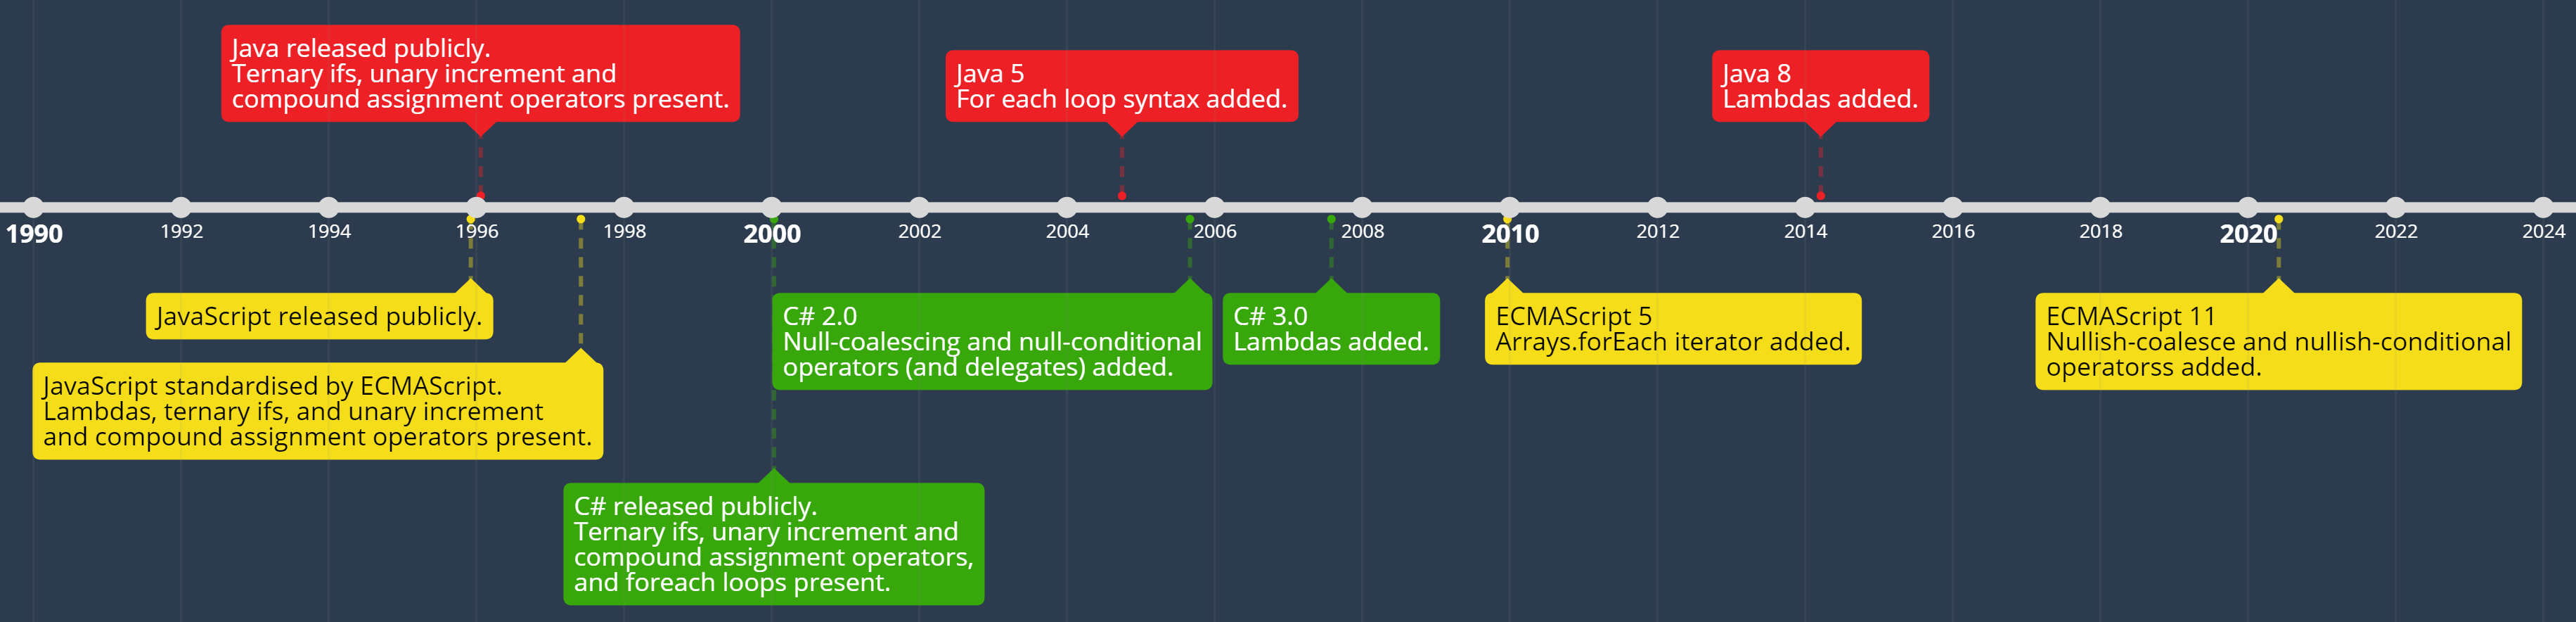
\includegraphics[width=1.5\textheight]{timeline}
        \caption{Timeline of the addition of advanced constructs to three modern languages.}
        \label{fig:timeline}
    \end{figure}
\end{landscape}
\newpage
\section{Study Design}
    \subsection{Constructs}
    \label{subsec:constructs}
    The section will give a more detail description of each of the constructs to be examined. The constructs were selected as they are all replaceable with simpler syntax (in most scenarios - lambdas being a occasional exception, see section \ref{subsec:lambdas}) and, together, they represent a range of commonality from long-used compound assignment and unary increment operators at one end of the scale to much newer additions such as the null-coalescing and -conditional operators. The constructs are as follows:
    \begin{itemize}
        \item Ternary/in-line If Statements
            \begin{itemize}
                \item Reduces the common \codeword{if} \dots \codeword{else} \dots pattern into a single line of the form \codeword{a ? b : c}, where \codeword{a} is a conditional expression, \codeword{b} is the body of the \codeword{if} and \codeword{c} is the body of the \codeword{else}. While it may be possible in some languages to have multiple statement in the `b' and `c' sections of a ternary, but standard syntax only permits a single statement.
            \end{itemize}
        \item Lambdas and Anonymous Functions
            \begin{itemize}
                \item A lambda expression is any expression involving a function used as an argument, just as in Lambda Calculus. Though this is not required, lambdas most often take the form of anonymous (unnamed) functions defined in-line. \citep{javaLambdas}.
            \end{itemize}
        \item Null-coalescing Operator
            \begin{itemize}
                \item Used to provide a default value in place of a null value. Replaces a null-check (using an if statement) with a single assignment of the form \newline\codeword{a = possiblyNullValue  ?? valueIfNull} where \codeword{a} is of a nullable type. \citep{cs5Spec}.
            \end{itemize}
        \item Null-conditional Operator
            \begin{itemize}
                \item Used to access a member or element of its operand \emph{if and only if} that operand evaluates to non-null. Otherwise, it returns null. \citep{cs6Spec}. This allows a member/element access operation to be carried out without a null-check on the base operand, only on the evaluated value.
            \end{itemize}
         \item Foreach Loops
            \begin{itemize}
                \item Used to simplify for loops for the purposes of iterating over an abstract data structure, usually a type of some form of collection of like objects; those that can be indexed into to retrieve an element. For example, in C\#, a \codeword{foreach} loop may be used to iterate over the elements of an instance of any class that implements the \codeword{IEnumerable} interface. The same applies to Java with its \codeword{Iterable} interface. In C\#, if \codeword{numList} is of type \codeword{List<int>}:
                \\
                \codeword{for (int i = 0; i < numList.Count; i++)}\\
                \{\\
                \hspace*{1cm}\codeword{total += numList[i];}\\
                \}
                \\\\
                Can be written as:\\
                \codeword{foreach (int num in numList)}\\
                \{\\
                \hspace*{1cm}\codeword{total += num;}\\
                \}
            \end{itemize}
        \item Unary Increment Operator
            \begin{itemize}
                \item Used to increment or decrement an integer variable by one. Often seen in for loops to increment the index variable.
                \item For example:\\
                \codeword{a = a + 1;}\\\\
                Can be written as:\\
                \codeword{a++;}
            \end{itemize}
        \item Compound Assignment Operators
            \begin{itemize}
                \item Used to effectively ``append'' to a variable's value, compressing three references to variables/literals into two. In most supporting languages, a compound assignment operator exists for all basic arithmetic operators, logic operators and some others (such as in string concatenation).
                \item For example:\\
                \codeword{a = a * 2;}\\\\
                Can be written as:\\
                \codeword{a *= 2}
            \end{itemize}
    \end{itemize}

    \subsection{Survey}
    \label{subsec:survey}
        One of the facets of this study was to capture and analyse the perceptions and thoughts of a number of professional software developers with regard to the constructs being examined. This was carried out using a survey, constructed following guidelines laid down by both published literature (\cite{goodSurveys1}, \cite{goodSurveys2}) as well as a small amount of grey literature provided by higher education bodies.
        \subsubsection{Questions}
        \label{subsubsec:surveyQuestions}
            Prior to designing, it was established that the survey must be able to provide insight that may help to answer the following questions:
            \begin{enumerate}
                \item Are the participants \emph{aware} of the constructs?
                \item Do the participants \emph{use} the constructs?
                \item Are participants \emph{encouraged to use} the constructs?
                \item Do the participants think these constructs are better for:
                \begin{enumerate}
                    \item brevity?
                    \item clarity?
                    \item code efficiency/performance?
                \end{enumerate}  
                \item Do the participants think that the constructs are better used in some languages than in others?
                \item Do participants rewrite code \emph{to use} or \emph{to not use} the constructs?
            \end{enumerate}
            
            Hypothesis/expected results
        \subsubsection{Participants}
            Participants were recruited passively from within the Information Systems Services department (ISS) within Lancaster University by means of a blanket email sent out to all teams and filtered down via regular communications channels within the department. This gathered 40 responses in total, 23 of which completed the survey and may be considered valid responses.
            
            Due to the distribution method, there is no guarantee that all respondents are software developers by profession, however, all participants had a minimum of one year of programming experience, nearly half falling into the 1-4 years of experience category, with three participants having between 10 and 14 years experience and the remaining 8 having over 20 years of experience. This statistic was the only personal data collected and does not identify participants.
        \subsubsection{Questions}
            The survey was created using Qualtrics, as provided by Lancaster University, and consisted of a maximum of 16 questions and a minimum of 2 questions (depending on certain answers).
            Participants were first asked to indicate which of the constructs they were aware of so that only questions and option relating to those constructs they were aware of were shown to them. For each construct they were of, participants were asked to a series of questions design to address the questions listed in section \ref{subsubsec:surveyQuestions}, focussing on: frequency of usage, reasons to and to not use each construct, perception on code performance, and perception of industry-wide usage per-language.
            
            Lastly, participants were asked if they had any further comments, which invited some very interesting points that will be discussed alongside the rest of the results in section \ref{subsec:results}.
    \subsection{Static Code Analysis}
        Static code analysis is concerned with checking programs and code for errors without the need to actually execute it. That is, a static code analysis tool will read the source code (or the compiled intermediary language in some cases), construct some form of abstract model of the program and then run a series of tests (often pattern-matching in nature) to detect well-known possible pit-falls, bugs, and problems \cite{staticCodeAnalysis}.

        These tools will often make recommendations on how source code may be improved in numerous way beyond explicit bugs and problems, such as stylistic improvement that make use of advanced syntax whatever given language is being analysed - advanced syntax akin to the constructs being examined here. Accordingly, static analysis tools were employed to investigate whether or not they made any recommendations for or against any of the constructs in question. SonarQube and Semgrep were selected for this purpose as they both support all three languages being subject to analysis, they are both under recent, active development, and because they both have free variants. Both tools were run against sample control code files and large open source repositories in the earlier mentioned three languages: C\#, JavaScript, and Java.
            
        \subsubsection{Sample Code Files}
            The sample code files were created to act as a baseline or control test to see if SonarQube or Semgrep made any note at all about the bare usage and/or inclusion of any of the constructs.

            Each file contains a bare (non-contextualised) example of each of the constructs placed directly alongside their `simple syntax' functionally equivalent counterparts. Each file is valid syntax for its language, and all of them may be executed, though none of them have a true entry point or way to actually \emph{run} the code within itself - the functions and methods are present purely to \emph{be present} so that they may be analysed by SonarQube and Semgrep. Though there are differences between the three languages, the form of the sample code was kept as similar as possible to preserve their purpose as control samples, without adding deliberately unusual syntax that may contaminate the output of SonarQube and Semgrep.
        \subsubsection{Open Source Repositories}
            Four large, open source code repositories were selected from GitHub to be analysed for this study, one each in C\# and JavaScript, and two in Java. The selection process was simple: 
    \subsection{Git Commit Analysis}
        To supplement the static analysis of the repositories, manual, by-hand analysis of the commits made to these repositories was also undertaken.

        The goal of this branch of the study was to understand if and how standards are being maintained within the repositories within reference to the constructs and to general style-keeping. This was carried out by cloning the repository and examining the commit history using \codeword{git log}. A list of keywords were run against the commit history using the \codeword{--grep=<pattern>} option to \codeword{git log}. The keywords used are listed below:
        
        \begin{center}
            \begin{tabular}{ | l | l | }
                \hline
                \textbf{General} & style \\
                \hline
                \textbf{Ternary} & ternary, conditional, \codeword{?:}, elvis \\
                \hline
                \textbf{Null coalesce/conditional} & null, coalesce, conditional, \codeword{??}, \codeword{?.}, \codeword{?[} \\
                \hline
                \textbf{Lambda} & lambda, arrow, \codeword{=>}, \codeword{->} \\
                \hline
                \textbf{For each} & foreach, for each \\
                \hline
                \textbf{Unary Operators} & unary, increment, decrement, ++, -{}- \\
                \hline
                \textbf{Compound Operators} & compound, assign, \codeword{+=}, \codeword{-=}, \codeword{*=}, \codeword{/=}, \codeword{|=}, \codeword{&=} \\
                \hline
            \end{tabular}
        \end{center}

        Some of these keywords generated cross-over between those meant to highlight changes around a particular construct, but this was unimportant as these keywords were only used to create a list of  `interesting' commits. Commits were deemed interesting if the commit message and/or description contained reference to any of the keywords in such a way that it seem plausible that a change was made regarding any relevant construct. For each commit in the resultant list, the changes were scrutinised closely to pick out changes made that: added, removed, altered, or commented on usage of any of the constructs. Each type of change was documented and counted per commit.

\newpage
\section{Results}
    \subsection{Survey}
    \label{subsec:results}
        As described in section \ref{subsec:survey}, a survey was conducted with a number of experienced professional software developers and programmers. This revealed a number of interesting patterns of usage (or lack of, therein) of the constructs, and some interesting perceptions that may prove useful in future research focussed on performance and usage in the wider industry.

        The following sections will detail the discovered patterns, grouped by the overarching category of information acquired in the survey.
        \subsubsection{Awareness}
            Awareness of the constructs was gathered by a simple multiple choice question with a binary yes/no for each. Participants could indicate whether or not were familiar with all, some, or none of the constructs.
            \\\newline
            Hypothesis: \textit{All participants will be aware of unary and compound operators, most will be aware of ternary/in-line if-statements and lambdas, some will be aware of null-coalesce, and few will be aware of null-conditionals.}
            \\\newline
            All participants were aware of unary operators and ternary/in-line if-statements, nearly all were aware of compound operators and lambdas, and most were aware of null-coalesce and null-conditional. Figure \ref{fig:awareness} shows these results in a graphic format.

            \begin{figure}[htbp]
                \centering
                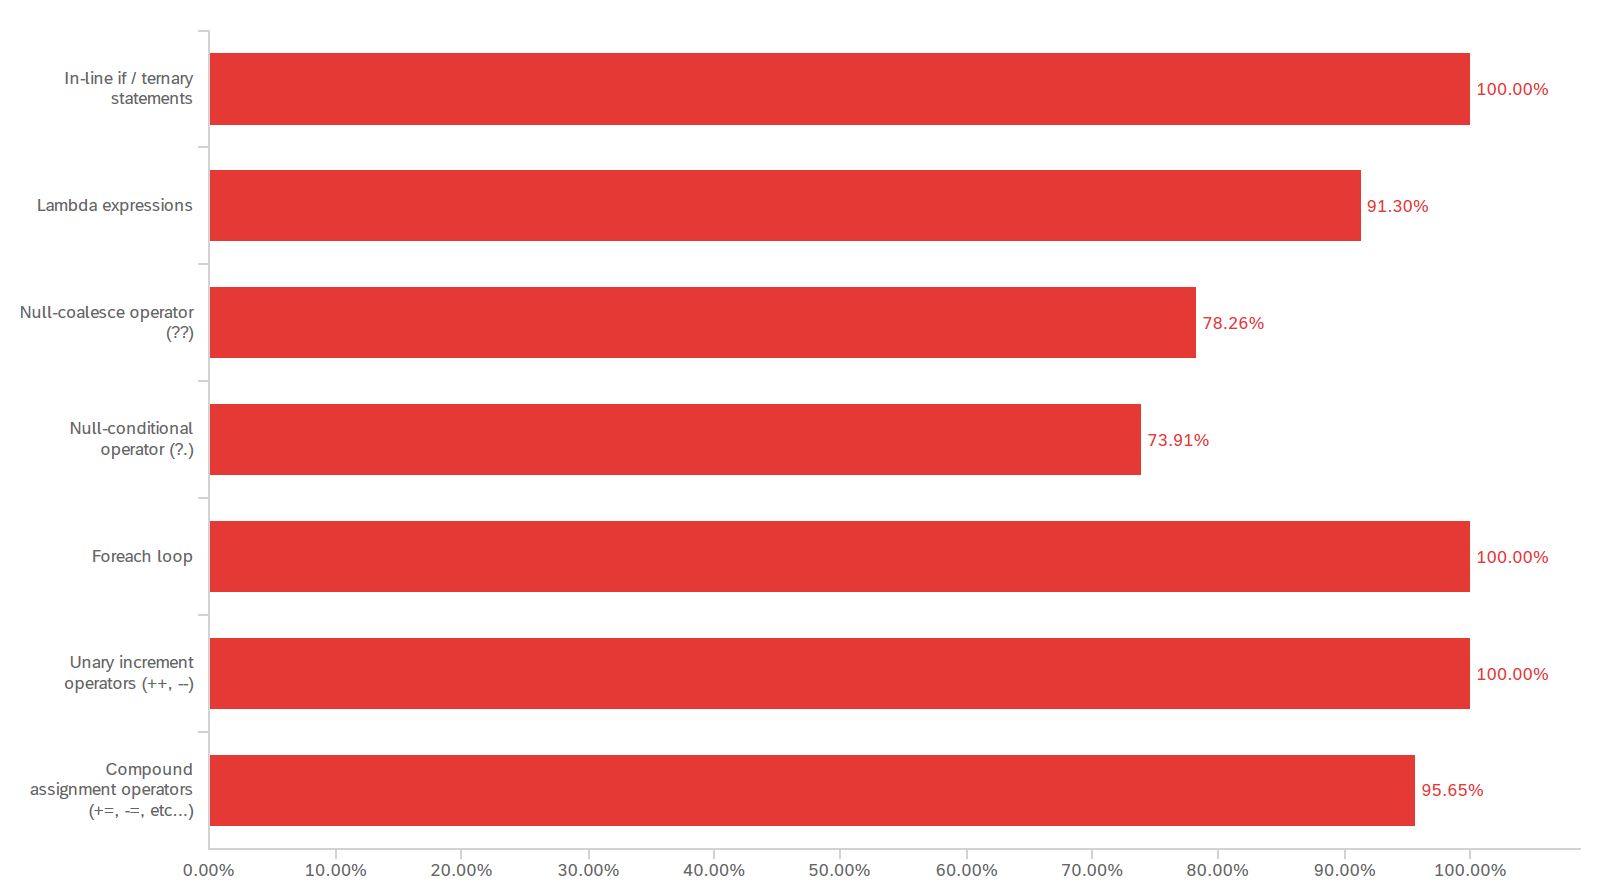
\includegraphics[width=0.8\textwidth]{awareness}
                \caption{Percentage of participants aware of each construct}
                \label{fig:awareness}
            \end{figure}

            The hypothesis was partially met, the most stand-out discrepancy being that though the relative position was as predicted, \emph{absolute} awareness of the null-coalesce and -conditional operators was markedly higher than expected. This can likely be attributed to the fact that participants were all from within ISS, where the  technology stack contains a significant amount of C\#, in which these operators are often seen. If the survey were repeated over more diverse and broad range of developers working in more varied technology stacks (for example, those focussed much more on Java, or C/C++), it is reasonable to assume that awareness of these operators would be less. This is a trend that is repeated elsewhere in the results set.
            It is also of note (if not significantly so) that not \emph{all} participants were aware of compound assignment operators, whereas all participants \emph{were} aware of ternaries - a ranking inverse to what was expected. However, the difference in the numbers are not statistically significant, comprising no more than one or two responses. To draw any conclusion from this datum would require it being replicated in a greater sample set.
        \subsubsection{Usage Frequency}
            To assess how often participants use each of the constructs, they were asked specifically: \textit{In places where they can be used, how often do you use each of these constructs in your code?}, that is, ``for every chance you \emph{could} use the construct, how often do you?''
            \\\newline
            Hypothesis: \textit{Unary and compound operators are used always, for each loops are used either always or frequently, ternaries and lambdas are used sometimes, and null-coalesce and null-conditional are used rarely.}
            \\\newline
            It was the extreme ends of the scales in this question that provided the most interesting results here. Firstly, and perhaps reassuringly, only one data point was recorded, for any construct, under the `never' option, with just one respondent indicating that they never use the null-coalesce operator. Conversely, `for each' was the most selected construct in the `always' category, with 44\% of participants selecting this option, followed closely by compound assignment operators at 41\%.

            Across all constructs, the majority of responses fell into the `frequently' category, holding 39\% of the total selections, with the `sometimes' category at 27\%. This general erring toward the more frequent end of the scale holds not only for the collective dataset but also for each construct when examined individually, as may be seen in figure \ref{fig:freqUse}

            \begin{figure}[htbp]
                \centering
                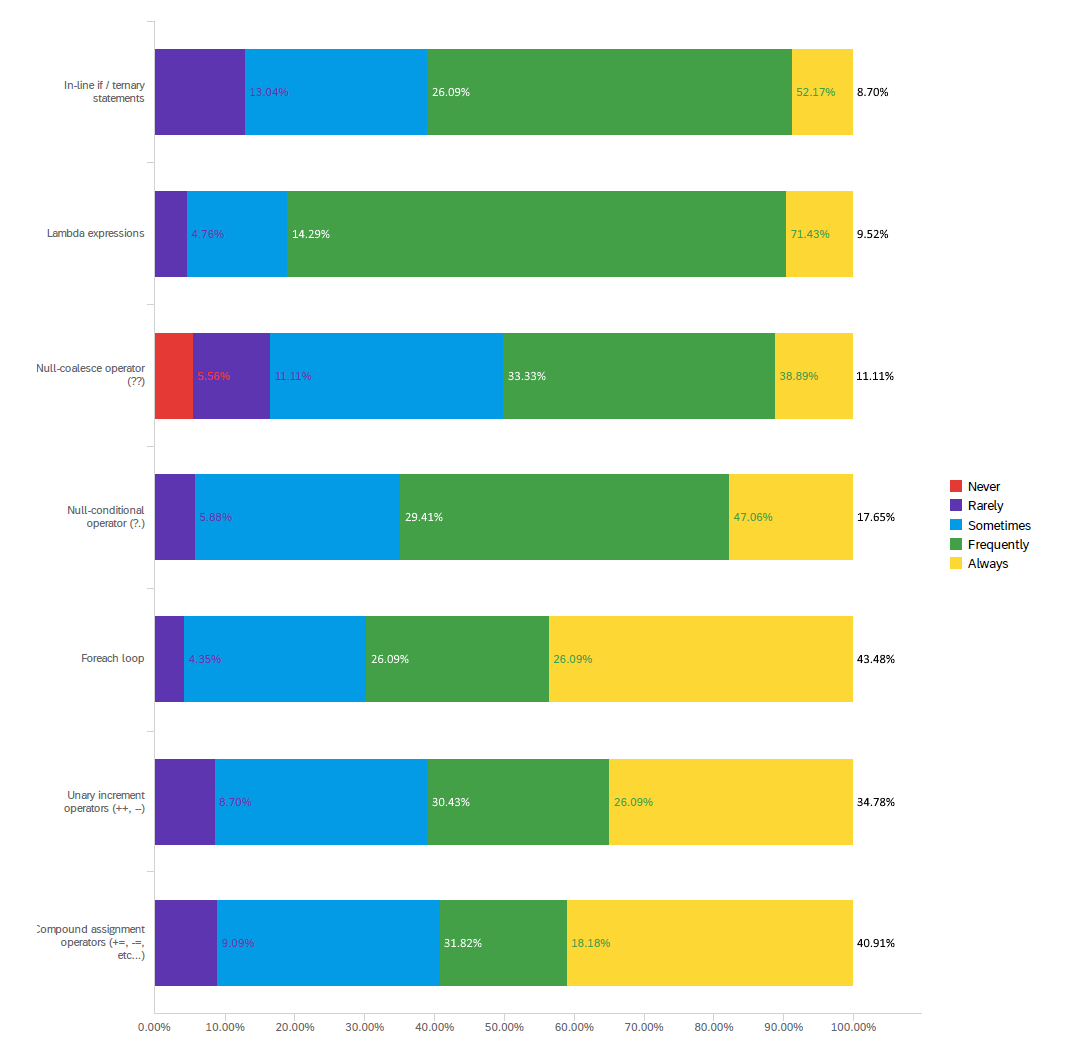
\includegraphics[width=0.8\textwidth]{freqUse}
                \caption{Frequency with which participants said they used advanced constructs, grouped by construct}
                \label{fig:freqUse}
            \end{figure}

            As is visible in figure \ref{fig:freqUse}, the usage of lambdas in moderation is the most agreed upon data point here, with just over 70\% of responses labelled `sometimes' for lambdas. This aligns with the hypothesis for lambdas. This is likely explainable by a variety of reasons, not least is the fact that lambdas are very powerful and complex structures, much more so than the other constructs being studied, and as such, the number of situations where they \emph{can} be used likely greatly exceeds the number situations where they \emph{should} be used. This distinction around lambdas becomes more apparent in later questions.
            Of note, again, is the misalignment of the hypothesis with the results of the null-coalesce and null-conditional operators. Although the numbers of participants familiar with these operators is fewer, those that were aware of them do not shy away from them, using them with comparatively similar frequency to the other constructs.
        \subsubsection{Reasons To Use}
            Participants were then asked to indicate \emph{why} they chose to use each given construct. The four options were presented:
            \begin{itemize}
                \item ``It is company style''
                \item ``It makes code clearer''
                \item ``It makes codes simpler''
                \item ``It makes code run faster''
            \end{itemize}
            All, some, or none of the options may have been selected. Where the exclusive option ``None of these'' was selected, participants were prompted to give their own reason.
            \\\newline
            Hypothesis: \textit{Style is a primary factor for usage of ternary if-statements, null-coalesce, null-conditional, for each, unary operators. Reasons of simplicity are also key for usage of lambdas, null-coalesce, null-conditional, for each, and unary and compound operators. Additionally, lambdas and for each make code clearer. Null-coalesce may also be used for reasons of speed/efficiency.}
            \\\newline

            `Well yes but actually no.'
        \subsubsection{Reasons To Not Use}
            []
        \subsubsection{Performance}
            []
        \subsubsection{Usage In Wider Industry}
            []
    \subsection{Static Code Analysis}
        []
        \subsubsection{Sample Code Files}
            Bugger all picked up, tools do not care
            \begin{itemize}
                \item Picked up basic for in place of JS for-to (not for/each)
            \end{itemize}
        \subsubsection{Real-World Code Bases}
            []
\newpage
\section{Conclusion}
\label{sec:conclusion}
    []
    \subsection{Review of Aims}
        The following list repeats the aims presented at the start of this report, with each aim followed by an overview of relevant results obtained.
        \begin{itemize}
            \item \textcolor{gray}{\textit{[]}}
                []
            \item \textcolor{gray}{\textit{[]}}
                []
            \item \textcolor{gray}{\textit{[]}}
                []
            \item \textcolor{gray}{\textit{[]}}
                []
            \item \textcolor{gray}{\textit{}}
                []
        \end{itemize}
    \subsection{Reflections}
        []
        \begin{itemize}
            \item survey: what does "complexity" mean? Computational? That'd be covered by slow/faster?
            \item GitHub repo selection: mistakenly thought it was `top of all repos for lang., it was not. (Check Tracy emails for reference and remedy, time permitting)'
        \end{itemize}

        
    \subsection{Negative Impacting Circumstances}
        The on-going coronavirus pandemic is still very much a factor in the lives us all. :(
    \subsection{Future Research}
        []
    \subsection{Closing Statement}
        []

\newpage
\bibliography{ref}
\newpage
\section*{Appendix}
    \subsection*{Appendix 1: []}
        []
    \subsection*{Appendix 2: []}
        []
\end{document}
